\section{Přehled databázových systémů a jejich historie}

Databázový systém (anglicky \upabbrevref{DBMS}) je soustava komplexního aplikačního vybavení, které je podloženo určitým teoretickým základem. Jeden bez druhého nemůže existovat (resp. může, což má ale za následek formální selhání \upabbrevref{DBMS} jako takového), a tak je nutné znát obě strany pomyslné databázové barikády. Databázový systém tedy tvoří:
\begin{enumerate}
\item Aplikační software, který je obvykle používán jako rozhraní pro přístup k databázi samotné.
\item Teorie, která formálně podkládá návrh databáze, organizaci dat a obsahuje algoritmickou stránku věci.
\end{enumerate}

Mějme na paměti, že obě částí databázových systémů se rozvíjely postupně a mnohdy metodou pokus - omyl. Obecně platí, že pokud selže teoretický základ, tak již ani sebelepší frontend nic nezmůže. V databázovém systému se objeví formální rozpor a jedinou cestou vpřed je začít znovu.

Hlavním úkolem \upabbrevref{DBMS} je poskytovat \textit{perzistentní uložení dat}, dále poskytnout svým uživatelům konzistentní rozhraní a případně nabídnout \textit{transa-kční zpracování dat}. Nutnto podotknout, že poslední bod nemusí být takovou samozřejmostí, jak by se mohlo zdát.

\subsection{Historie databázových systémů}
Potřeba organizace dat je stará jako lidstvo samo. Již staří Egypťané si vedli podrobné záznamy o výběru daní, stavbách chrámů a jiných činnostech. Zde můžeme hovořit o databázích založených na souborech.

\subsubsection{Databáze založené na souborech}
Souborem může být například papyrus, hliněná destička nebo (lépe) papír. Na papíře můžete být napsány v řádcích nějaké záznamy. Například seznam dlužníků nějakého podnikatele. \textit{Vytvoření} takového seznamu je vskutku \textit{lehké}. Představme si, že dlužník uprostřed seznamu splatil svůj dluh a bude ze seznamu vyškrtnut. Místo něj v seznamu vznikne prázdné místo. Zbytek seznamu se následně musí zkonsolidovat (přepsat na nový papír), aby vypadal konzistentně. Odtud plyne určitá \textit{těžkopádnost} vyplývající z definice souboru a z určité \textit{nízkoúrovňovosti} práce s ním. Přitom souborem může být myšlen i soubor na disku počítače.

Představme si navíc, že daný podnikatel si vede další soubor se seznamem, kde si u každého dlužníka značí jeho adresu, aby jej mohl v případě nutnosti navštívit. Jméno dlužníka tedy uchováva hned na dvou seznamech, přitom je přirozeně jasné, že stačí dlužníka evidovat jednou a poté se na něj \enquote{odkazovat.} \textit{Redundace dat} je tedy zřejmá.

\subsubsection{Databáze založené na síťovém modelu}
Průkopníkem této oblasti byl Charles Bachman. Aktuálně se toto paradigma považuje za dávno překonané, nicméně pro časy budoucí poskytlo několik dob-rých poznatků. Typicky \enquote{síťový} databázový systém je tvoří mj. i:
\begin{enumerate}
\item \textit{Záznamy}, které mají určitý \textit{typ}. Ten deklaruje, jaké \textit{atributy} daný zázna obsahuje. Atributy mohou nabývat různých hodnot.
\item \textit{Odkazy}, které reprezentují \textit{vztahy} mezi jednotlivými záznamy.
\end{enumerate}
Obecně se ví, že databázové systémy tohoto typu mohou poskytovat velmi rychlé prostředky pro získávání jednoduchých dat, ale na druhou stranu na komplexnější data se dotazuje hůře. Tvorba dat není rovněž jednoduchá, protože práce s odkazy požaduje vyšší míru sofistikace.

\begin{figure}
\centering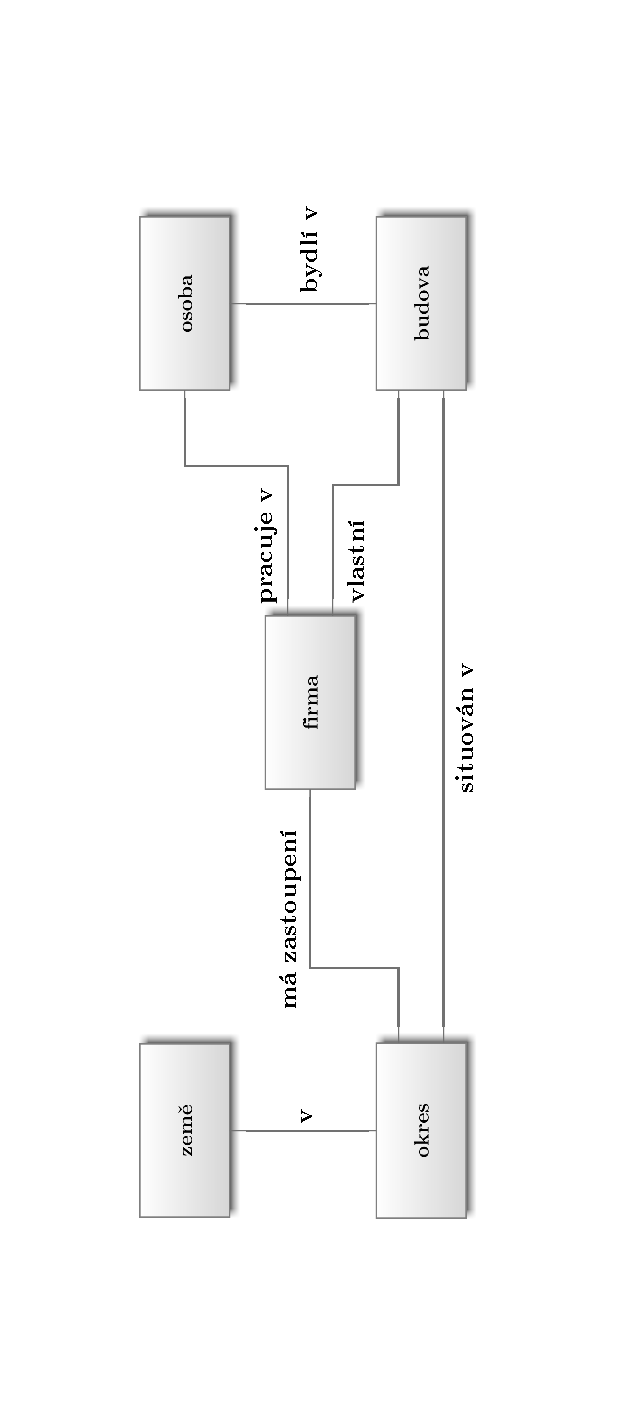
\includegraphics[angle=-90,width=14cm]{graphics/01-sitovy}
\caption{Datový model s obousměrnými odkazy}
\end{figure}

\begin{figure}
\centering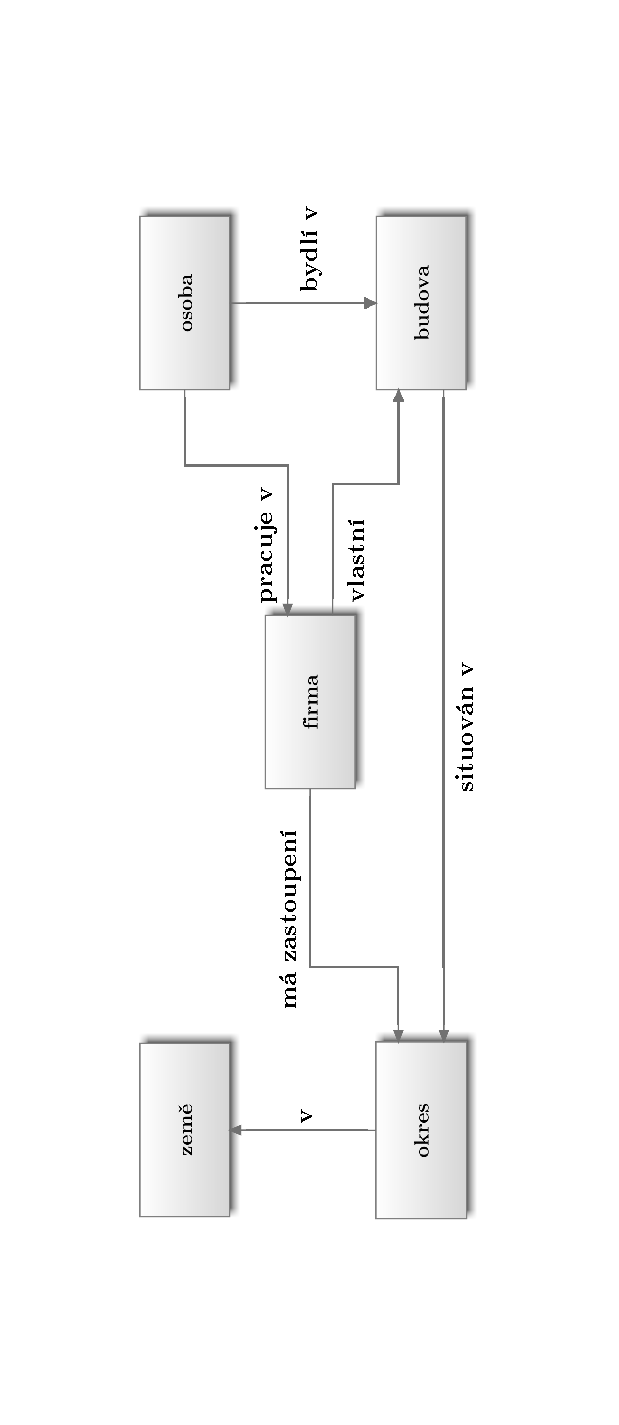
\includegraphics[angle=-90,width=14cm]{graphics/01-sitovy2}
\caption{Datový model s jednosměrnými odkazy}
\end{figure}

\subsubsection{Databáze založené na hierarchickém modelu}
Jedná se o speciální typ síťového modelu, kde bylo úmyslem tento model zjednodušit. Výsledkem bylo vytvoření hierarchie v záznamech a odkazech ve formě stromu\footnote{Strom je jednou ze základních grafových struktur. Jedná se o (neorientovaný) graf bez kružnic. Více napoví \citep[str. 91 -- 96]{cormen:algorithms}.}.

\subsubsection{Databáze založené na objektovém modelu}
V objektovém modelu jsou hlavní prvky, jenž reprezentují data, \textit{objekty}, tery serializované entity, které lze interpretovat pomocí nějakého vyššího programovacího jazyka. Prvním jazykem podporujícím takovéto pojetí byl Common Lisp.

\subsubsection{Databáze založené na relačním modelu}
Jedná se o aktuálně používaný model, který přináší určité výhody. Primárním nosičem informace v tomto modelu jsou \textit{relace} (poněkud amatérsky je můžeme nazývat také tabulkami). Základy tohoto modelu položil Edgar Codd v roce 1970.

% obrázek struktury databáze.

\section{Relační model dat}
Model má 3 základní komponenty:
\begin{enumerate}
\item \textit{Struktury}, které uchovávají data a reprezentují výsledky dotazů.
\item \textit{Integritní omezení}, která popisují vztahy mezi daty, které musí být splněny. Integritní omezení jsou v podstatě formule. Tato omezení slouží k popisu toho, jak mají data vypadat, slouži k odstranění jejich chyb.
\item \textit{Manipulativní formalismy}, které říkají jak z uložených dat získat jiná data určitými operacemi.
\end{enumerate}
Relační mode je konkrétním modelem dat, avšak modely jako takové lzde rozdělit do dvou skupin, tedy:
\begin{enumerate}
\item Abstraktní modely dat, které poskytují vyčerpávající logické definice datových struktur nebo operací s daty. Ty dohromady tvoří abstraktní formalismus. Tedy jakýsi abstraktní stroj, se kterým může uživatel operovat.
\item Konkrétní modely, pracující s persistentními daty.
\end{enumerate}

\section{Struktura relačních dat}
Základním kamenem dat jsou tzv. \enquote{datové tabulky}, které obsahují záhlaví a další data.
\begin{enumerate}
\item Záhlaví (viz. tabulka \ref{tab:zahlavi}) je množina atributů a jejich typů. U tabulky se seznamem zamě-stnanců může být atributem například jméno zaměstnance atp.
\item Vlastní data (neboli tělo) tabulky by u takovéto tabulky představovala data samotných zaměstnanců.
\end{enumerate}

\begin{table}
\caption{Záhlaví tabulky}\label{tab:zahlavi}
\begin{center}
\begin{tabular}{|c|c|c|}
\hline
ID & JMÉNO & ADRESA \\
\hline
15 & Vyacheslav Drsoň & Peklo, 666 \\
\hline
\vdots & \vdots & \vdots \\
\hline
\end{tabular}
\end{center}
\end{table}

\subsection{Požadavky na tabulky}
\begin{enumerate}
\item\label{enum:first_re} Řádky by neměly mít žádné pořadí. Tabulka by měla být chápána jako množina řádků. A v množině na pořadí nezáleží.
\item To samé platí pro sloupce.
\item Z definice množiny také vyplývá, že tabulka by neměla obsahovat identické řádky. Tento požadavek není v mnoha \upabbrevref{DBMS} splněn.
\item V každém poli uvnitř tabulky je právě jedna hodnota daného typu.(SQL porušuje nedefinovanou hodnotou)
\item\label{enum:last_re} Všechny atributy jsou regulární.
\end{enumerate}
Tyto požadavky formuloval C.~J.~Date.
Pokud tabulka splňuje body \ref{enum:first_re} až \ref{enum:last_re}, pak je v 1. normální formě.

Zavedli jsme si několik pojmů jako \textit{atribut} a tak dále. Formalizujme je nyní přesněji:
\begin{description}
\item[Atribut] popisuje účel daného sloupce v tabulce, je to jméno sloupce.
\item[Typ] říká, jakých hodnot může atribut nabývat.
\item[Doména] je množinou všech možných hodnot daného typu. Tedy například nějaký pomyslný typ\upinlinecode{SQL}{!}{BOOL} by mohl mít doménu ve tvaru: $$
\dom(BOOL) = \left\{ true, false \right\}
$$
\end{description}

\subsection{Relační schéma}
Již dříve jsme si uvedli pojem \textit{záhlaví tabulky}, avšak ten byl poněkud vágní. Relační schéma je jeho analogií s přesnější definicí.
\begin{uptheorem}[Relační schéma]
Mějme množinu atributů $Y$ a množinu typů $T$ Následně platí, relační schéma $R$ je množina definovaná jako:
$$
R = \left\{ \left\langle y, t \right\rangle \; | \; y \in Y, t \in T \right\}
$$
\end{uptheorem}
Proveďme dohodu, že typ atributu $y$ budeme zapisovat také jako $\typ(y)$ a analogicky doménu pro každý typ budeme značit jako $\dom(y)$.

\subsection{Obecné kartézské součiny}
Mějme následující systém množin:
$$
\left\{ A_{i} \; | \; i \in I \right\}
$$
kde $I$ je tzv. indexní (a libovolná) množina a $i$ je index z této množiny. Kartézský součin $A_{i} (i \in I)$ se značí $\prod_{i \in I} A_{i}$ a je definován jako množina zobrazení $f: I \rightarrow \bigcup_{i \in I} A_{i}$, kde $f_{i} \in A_{i}$ pro každý $i \in I$.

Prvky $\prod_{i \in I} A_{i}$ jsou zobrazení, nezáleží v nich na pořadí indexů.
\begin{upexample}[Kartézský součin]
Vypočítejme kartézský součin množin $A$ a $B$, tedy $A \times B$ se zadáníms:
$$
A = \left\{ a, b, c \right\}, \quad B = \left\{ 10, 10 \right\}, \quad I = \left\{ 1, 2 \right\}, \quad A_{1} = A, \quad A_{2} = B
$$
Následně řešení:
$$
\prod_{i \in \left\{ 1, 2 \right\}} A_{i} = \left\{ \left\langle a, 10 \right\rangle, \left\langle b, 10 \right\rangle. \left\langle a, 20 \right\rangle, \left\langle b, 20 \right\rangle \right\}\footnote{Zmíněnou rovnost nutno brát mírně s rezervou, protože formálně výsledkem kartézského součinu je množina zobrazení, nikoliv uspořádaných množin.}
$$
\end{upexample}

\begin{upexample}[Kartézský součin s tečkovou indexní množinou]
Mějme $I = \left\{ \bullet \right\}$ a $A_{\bullet}$. Pak platí, že $\prod_{i \in I} A_{\bullet} = A_{\bullet}$ s funkcí $f: \left\{ \bullet \right\} \rightarrow A_{\bullet}$.
\end{upexample}

\begin{upexample}[Kartézský součin žádné množiny]
Nechť $I = \varnothing$. Pak $\prod_{i \in I} A_{i} = \left\{ \varnothing \right\}$ s funkcí $f: \varnothing \rightarrow \varnothing$.
\end{upexample}

\subsection{Relace nad relačním schématem}
\begin{uptheorem}[Relace nad relačním schématem]
Mějme relační schéma $R$, pak relace nad $R$ je libovolná konečná podmnožina na kartézském součinu domén atributů z $R$, tedy
$$
\mathcal{D} \subseteq \prod_{y \in R} \dom(y)
$$
Relace v takovémto pojetí přibližně odpovídá vágnějšmu pojmu \textit{tabulka}. Součin lze pochopitelně také rozepsat. Obsahuje-li relační schéma $R$ celkem $n$ atributů, pak platí, že:
$$
\mathcal{D} \subseteq \dom(A_{1}) \times \cdots \times \dom(A_{n})
$$
Pozorný čtenář určitě pozoruje, že každá relace (tabulka) může mít určitý maximáln možný počet řádků. Matematicky:
$$
\left|\mathcal{D}\right| = \left|dom(A_{1})\right| \times \cdots \times \left|dom(A_{n})\right|
$$
Relaci lze také označit jako dvojici $\left\langle \mathcal{D}, R \right\rangle$. Tato dvojice takřak kompletně popisuje tabulku.
\end{uptheorem}
Každý prvek relace (tabulky) se nazývá n-tice. To je analogické vzhledem k matematickému pojetí relaci jako takových. Matematické relace též obsahují n-tice.

\subsubsection{Speciální případy relací}
\begin{enumerate}
\item Prázdná relace (tabulka) nad $R$, tedy $\left\langle \varnothing, R \right\rangle$.
\item Tabulka \enquote{dum}, tedy $\left\langle \varnothing, \varnothing \right\rangle$.
\item Tabulka \enquote{dee}, tedy $\left\langle \left\{ \varnothing \right\}, \varnothing \right\rangle$.
\end{enumerate}

\section{Tutorial D}
Programovací jazyk Tutorial D formuje opozici vůči mnohem známějšímu a v praxi používanějšímu \upabbrevref{SQL}. Tutorial D má jedinou funkční a (víceménně) použitelnou implementaci známou jako Rel. Frontend Rel je naprogram v jazyce Java a jeho prostředí vypadá bohužel hrůzostrašně. Rel je silně staticky typovaný, nemá konverze typů. Obsahuje typy:
\begin{description}
\item[Skalární], které jsou opozitem hodnotových typů ze známějších jazyků a patří sem například\upinlinecode{TutorialD}{!}{BOOLEAN},\upinlinecode{TutorialD}{!}{INTEGER} nebo\upinlinecode{TutorialD}{!}{STRING}.
\item[N-ticové], které jsou dané jmény atributů a jejich typy.
\end{description}
Dále Rel disponuje \textit{relačním} typem, který představuje instance tabulek. Rel pracuje s proměnnými konstruktivně, proměnné nemohou měnit svůj obsah (hodnotu), místo toho se vytváří nová proměnná s novou hodnotou. Každá proměnná má tedy svůj typ.

\subsection{Výrazy versus příkazy}
Výrazem v Tutorial D (resp. v Rel) je například prostá logická rovnost hodnot. Výraz může mít nějaký výsledek. Příkaz se od výrazu liší tak, že končí středníkem a obvykle obsahuje volání nějaké funkce.
\begin{upcode}{Výraz a příkaz (Tutorial D)}{}{TutorialD}
/* výraz */
666 = 6661215
/* příkaz */
WRITELN(10 = 20);
\end{upcode}

\subsection{N-tice jako hodnoty}
V Tutorial D lze přímočaře vytváře řádky relací a považovat je za hodnoty, viz. kód \ref{code:valstuple}.
\begin{upcode}{Základy n-tic (Tutorial D)}{code:valstuple}{TutorialD}
/* prázdná n-tice */
TUPLE {}
/* n-tice včetně dat */
TUPLE {id 666, name "Vilík", lab 5077}
/* rovnost n-tic */
WRITELN(TUPLE {id 666, name "Vilík", lab 5077} = TUPLE {id 007, name "James Bond", lab 1111});
/* vnořené n-tice */
TUPLE {id 666, TUPLE {jmeno "Vilík" prijmeni "Devil"}, lab 5077}
\end{upcode}
Z n-tic lze pochopitelně získávat hodnoty nebo n-tice sjednocovat, zúžovat a tak podobně.
\begin{upcode}{Operace s n-ticemi (Tutorial D)}{}{TutorialD}
/* vypíše hodnoty atributů id a lab (zúžení n-tice) */
TUPLE {id 666, TUPLE {jmeno "Vilík" prijmeni "Devil"}, lab 5077} {id, lab}
/* vypíše vše kromě lab (zúžení n-tice) */
TUPLE {id 666, TUPLE {jmeno "Vilík" prijmeni "Devil"}, lab 5077} {ALL BUT lab}

/* sjednocení n-tic */
TUPLE {id 666, jmeno "Vilík"} UNION TUPLE {jmeno "Vilík", lab 5077}

/* přejmenování atributů n-tice */
TUPLE {id 666, jmeno "Vilík"} RENAME (id AS cislo, jmeno AS name)
\end{upcode}
Sjednocení n-tic bere dvě n-tice, které se shodují na nějakém atributu a ve výsledku se objeví konkatenace n-tic s jedním výskytem společného atributu. Kompozice n-tic funguje obdobně jako sjednocení, avšak ve výsledku se společné atributy vůbec neobjeví.
\begin{upcode}{Další operace s n-ticemi (Tutorial D)}{}{TutorialD}
/* rozšíření n-tice */
EXTEND TUPLE {id 666, jmeno "Vilík"} ADD (5077 AS lab)
/* aktualizace hodnot v n-tici */
UPDATE TUPLE {id 666, jmeno "Vilík"} (jmeno := "God")
\end{upcode}

\subsection{Relace v Tutorial D}
Tutorial D (potažmo Rel) samozřejmě podpruje relace.
\begin{upcode}{Operace s relacemi (Tutorial D)}{}{TutorialD}
/* relace s několika n-ticemi*/
RELATION {
	TUPLE {id 666, jmeno "Vilík"},
	TUPLE {id 007, jmeno "Bond"}
}
/* vytvoření relace jakožto typu */
VAR seznam_lidi BASE RELATION {id INTEGER, jmeno STRING} KEY {id};
\end{upcode}